\documentclass[11pt,a4paper]{article}
\usepackage[utf8]{inputenc}
\usepackage[spanish]{babel}
\usepackage{amsmath, amssymb}
\usepackage{graphicx}
\usepackage[margin=2.5cm]{geometry}
\usepackage{fancyhdr}
\usepackage{tcolorbox}
\usepackage{enumitem}

\definecolor{UCBblue}{RGB}{0, 51, 153}
\definecolor{UCBgray}{RGB}{100, 100, 100}
\definecolor{UCBred}{RGB}{153, 0, 0}

\pagestyle{fancy}
\fancyhf{}
\fancyhead[L]{\textcolor{UCBblue}{\textbf{Ingeniería Mecatrónica - UCB Tarija}}}
\fancyhead[R]{\textcolor{UCBgray}{Taller de Nivelación - Módulos 1 \& 2}}
\fancyfoot[C]{\thepage}
\renewcommand{\headrulewidth}{0.4pt}
\renewcommand{\headrule}{\hbox to\headwidth{\color{UCBblue}\leaders\hrule height \headrulewidth\hfill}}

\begin{document}

\begin{center}
    {\Large \textbf{\textcolor{UCBblue}{Guía de Modelado Analítico: Sistematización de Redes de Potencia}}}\\
    \vspace{0.3cm}
    {\large \textbf{Fase CDIO: Concebir (Fundamentos y Definiciones Exactas)}}\\
    \vspace{0.5cm}
    \textbf{Estudiante:} \rule{8cm}{0.4pt} \quad \textbf{Fecha:} \rule{3cm}{0.4pt}
\end{center}

\vspace{0.3cm}

\section*{1. Glosario Físico-Matemático Fundamental}
Para evitar que el álgebra lineal se reduzca a la manipulación abstracta de números, establecemos las siguientes definiciones rectoras para el modelado de hardware:

\begin{itemize}
    \item \textbf{Ley de Voltajes de Kirchhoff (LVK):} Es el principio de conservación de la energía en un circuito cerrado. La energía suministrada por las fuentes activas ($\mathbf{V}$) es exactamente igual a la energía disipada térmicamente por los elementos pasivos ($\mathbf{R}$).
    \item \textbf{La Matriz ($\mathbf{R}$) y el Vector ($\mathbf{I}$):} $\mathbf{R}$ no es una tabla de números, es el \textit{mapa topológico} que cuantifica la oposición estructural de la red. $\mathbf{I}$ es el \textit{vector de estado}, nuestra incógnita principal que dictará el flujo real de electrones hacia los actuadores.
    \item \textbf{El Determinante ($\det(\mathbf{R})$):} Escalar matemático que define la existencia de un punto de equilibrio único. Si $\det(\mathbf{R}) = 0$ (Matriz Singular), el modelo alerta de un \textbf{cortocircuito ideal} (corriente tendiente a infinito) o un conflicto entre fuentes de voltaje.
    \item \textbf{Regla de Cramer:} Método analítico que explora la sensibilidad de una variable de estado individual ($I_k$) dividiendo el determinante modificado ($\det(\mathbf{R}_k)$) entre el determinante topológico global ($\det(\mathbf{R})$).
\end{itemize}

\section*{2. Escalonamiento del Determinante: De $2\times2$ a $3\times3$}

Para comprender el algoritmo, iniciamos con la topología mínima funcional.

\begin{tcolorbox}[colback=blue!5!white,colframe=UCBblue,title=\textbf{A. Concepto Base (Matriz $2\times2$)}]
Para una red de dos mallas, el determinante nace de la resta de los productos diagonales (producto cruzado principal menos secundario):
$$ \mathbf{R} = \begin{bmatrix} a & b \\ c & d \end{bmatrix} \implies \det(\mathbf{R}) = (a \cdot d) - (b \cdot c) $$
\end{tcolorbox}

\begin{tcolorbox}[colback=blue!5!white,colframe=UCBblue,title=\textbf{B. Expansión Visual a $3\times3$ (Regla de Sarrus)}]
La Regla de Sarrus sistematiza el cálculo para tres mallas. Al duplicar las dos primeras columnas, se suman los productos de las tres diagonales descendentes y se restan los productos de las tres diagonales ascendentes.
\textbf{Limitación Crítica:} Este patrón visual \textit{solo es válido para matrices de $3\times3$}. Carece de validez matemática para dimensiones $4\times4$ o superiores, donde el ingeniero debe emplear expansión por cofactores o algoritmos de triangulación (Ej. Gauss/LU en Python).
\end{tcolorbox}

\newpage

\section*{3. Desarrollo Analítico: Misión de Ingeniería}

\begin{figure}[h!]
    \centering
    \framebox[14cm][c]{\rule{0pt}{6cm} 
    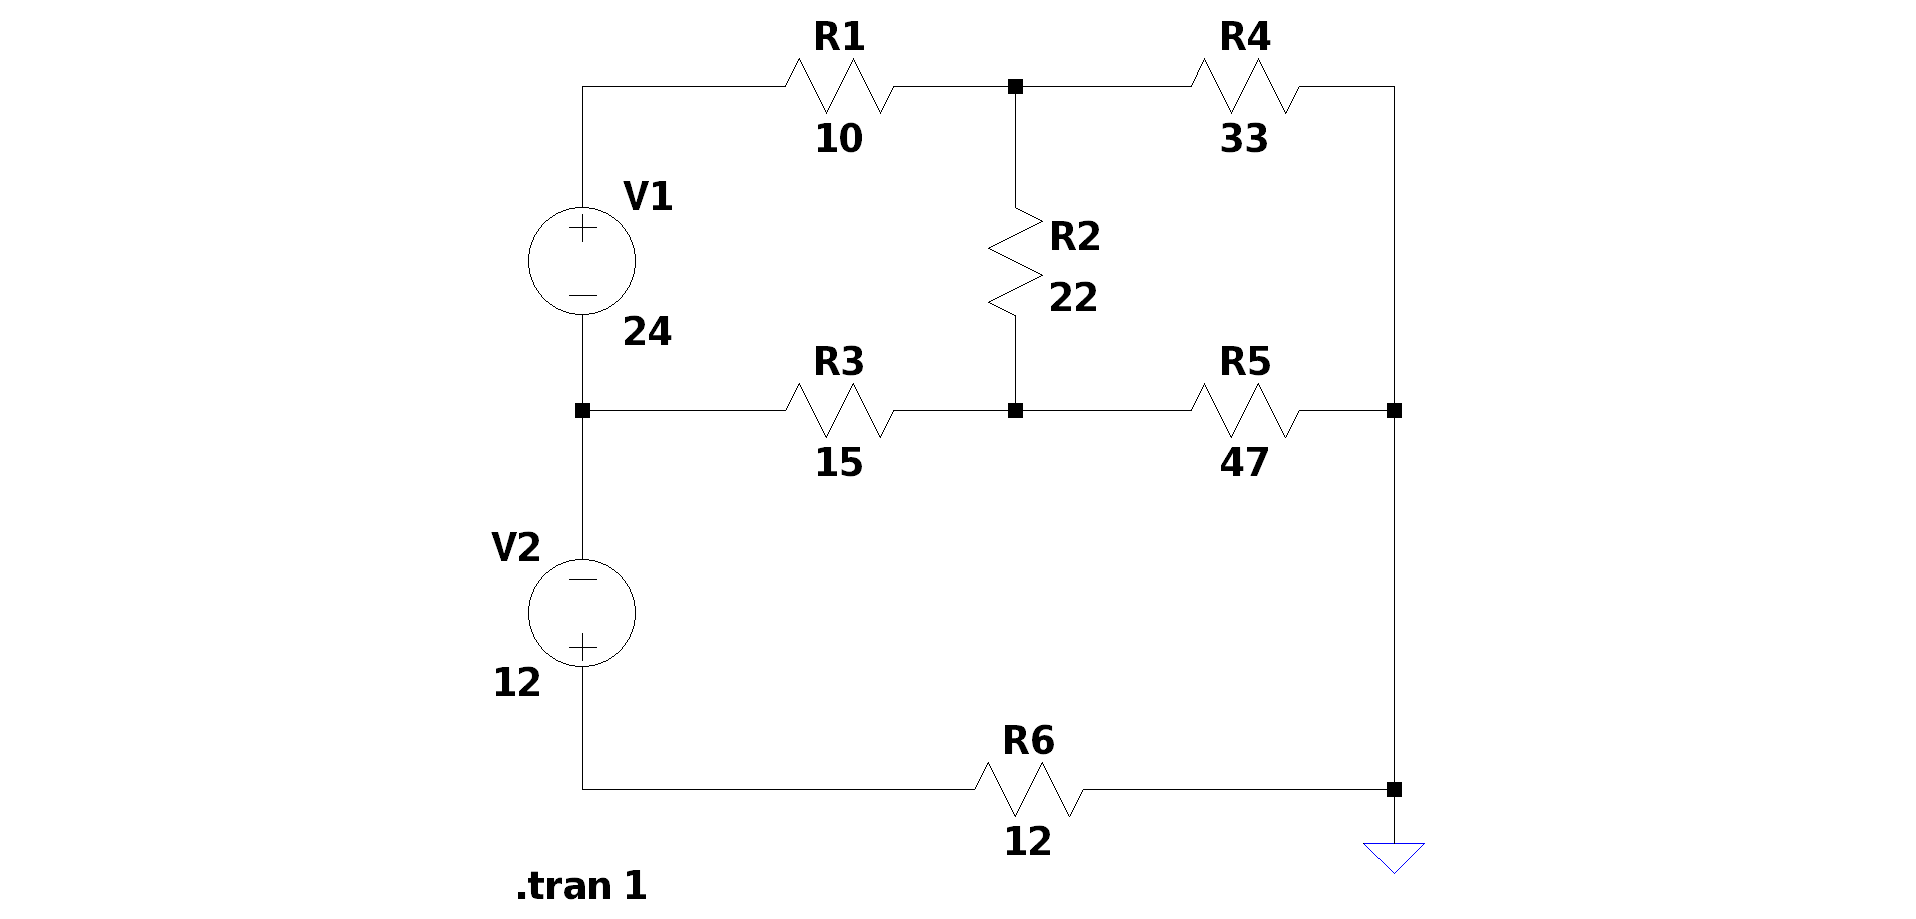
\includegraphics{schematic.png}
    }
    \caption{Topología coplanar de la red de distribución de potencia mecatrónica.}
\end{figure}

Considere la topología superior y aplique LVK para formular el sistema $\mathbf{R}\mathbf{I} = \mathbf{V}$ asumiendo $R_1=10\Omega, R_2=22\Omega, R_3=15\Omega, R_4=33\Omega, R_5=47\Omega, R_6=12\Omega$ y $V_{s1}=24V, V_{s2}=0V, V_{s3}=-12V$.

\textbf{A.} Ensamble la Matriz $\mathbf{R}$ garantizando la simetría y positividad diagonal:
\vspace{0.3cm}
$$
\begin{bmatrix}
 \dots \dots \dots & \dots \dots & \dots \dots \\
 \dots \dots \dots & \dots \dots \dots & \dots \dots \\
 \dots \dots \dots & \dots \dots \dots & \dots \dots \dots
\end{bmatrix}
\begin{bmatrix}
 I_1 \\
 I_2 \\
 I_3
\end{bmatrix}
=
\begin{bmatrix}
 \dots \dots \\
 \dots \dots \\
 \dots \dots
\end{bmatrix}
$$
\vspace{0.3cm}

\textbf{B.} Reemplace los parámetros por sus valores nominales y evalúe el determinante principal de la matriz mediante la \textbf{Regla de Sarrus}.

\begin{tcolorbox}[colback=white,colframe=UCBgray,height=4.5cm,valign=top]
\textit{Desarrollo analítico de Sarrus (Demostrar diagonales positivas y negativas):}
\end{tcolorbox}

\textbf{C.} Empleando la \textbf{Regla de Cramer}, sustituya la columna 1 de $\mathbf{R}$ por el vector $\mathbf{V}$, y calcule $I_1 = \frac{\det(\mathbf{R}_1)}{\det(\mathbf{R})}$.

\begin{tcolorbox}[colback=white,colframe=UCBgray,height=4cm,valign=top]
\textit{Cálculo analítico del Lazo 1:}
\end{tcolorbox}

\end{document}
